%----------------------------------------------------------------------------
\chapter{Elérhető telemanipulátorok}
\label{sec:LatexTools}
%----------------------------------------------------------------------------

A telemanipulátor egy olyan robotikai rendszer, amely lehetővé teszi egy távoli operátor számára, hogy távolról irányítsa és manipulálja a robotkarot vagy manipulátort. Ez a rendszer általában két fő részből áll: a távoli operátor konzoljából és a fizikai manipulátorból, amelyet általában egy robotkar vagy robotikai kar alkot.

A telemanipulátor rendszer célja, hogy a távoli operátor lehetőséget kapjon a távoli helyen történő munkavégzésre, amely lehet veszélyes környezet, távoli terület vagy olyan hely, ahová az ember nem férhet hozzá. A távoli operátor a konzol segítségével ad utasításokat a manipulátornak, amelyeket a robotkar vagy a manipulátor végrehajt a távoli helyen. Ennek eredményeként a távoli operátor képes manipulálni, mozgatni vagy érinteni tárgyakat a távoli helyen.

A telemanipulátorok széles körben alkalmazhatók különböző iparágakban és területeken. Például az űrkutatásban és az űrszemétszedésben használják a távoli helyen történő műveletek elvégzésére. Az orvostudományban telemanipulátorok segítségével végezhetnek távoli műtéteket és beavatkozásokat. Az ipari gyártásban használják a távoli manipulációt és a precíz munkafolyamatokat.

A telemanipulátor rendszerek különböző szenzorokat és eszközöket használnak, például képfeldolgozást, erőérzékelést és távérzékelést, hogy pontosabb és intuitívabb vezérlést biztosítsanak a távoli operátor számára. Az előrehaladó technológiák, például a virtuális valóság és a távérzékelés, további lehetőségeket kínálnak a telemanipuláció területén.

A telemanipulátor rendszerek lehetővé teszik az ember és a robot együttműködését, és hozzájárulnak a távoli helyeken történő feladatok hatékony és biztonságos elvégzéséhez. Ezáltal a telemanipuláció előnyös lehet olyan helyzetekben, ahol emberi jelenlét nem kívánatos vagy nem lehetséges, de mégis szükség van az emberi kézügyességre és irányításra.
\section{Telemanipulátorok az iparban}
%----------------------------------------------------------------------------
\section{Telemanipulátor az orvosi robotok vezérlésére}
%----------------------------------------------------------------------------
\section{Hat szabadság fokú telemanipulátor}
%----------------------------------------------------------------------------
Szakdolgozatomban bemutatott telemanipulátor egy egyszerű egytagú karokból és csuklókból összeállított eszköz. Az eszköz elkészítésének koncepciója, hogy a hatodik csuklóra helyezhető legyen egy geometria, amelynek a TCP-jának térben való elmozdulását rögzítsem a csuklószögek mérésével. Az alábbi képen is látható (\ref{fig:Szakdoga_csipeszes}) az elkészített eszköz.

\begin{figure}[!ht]
\centering
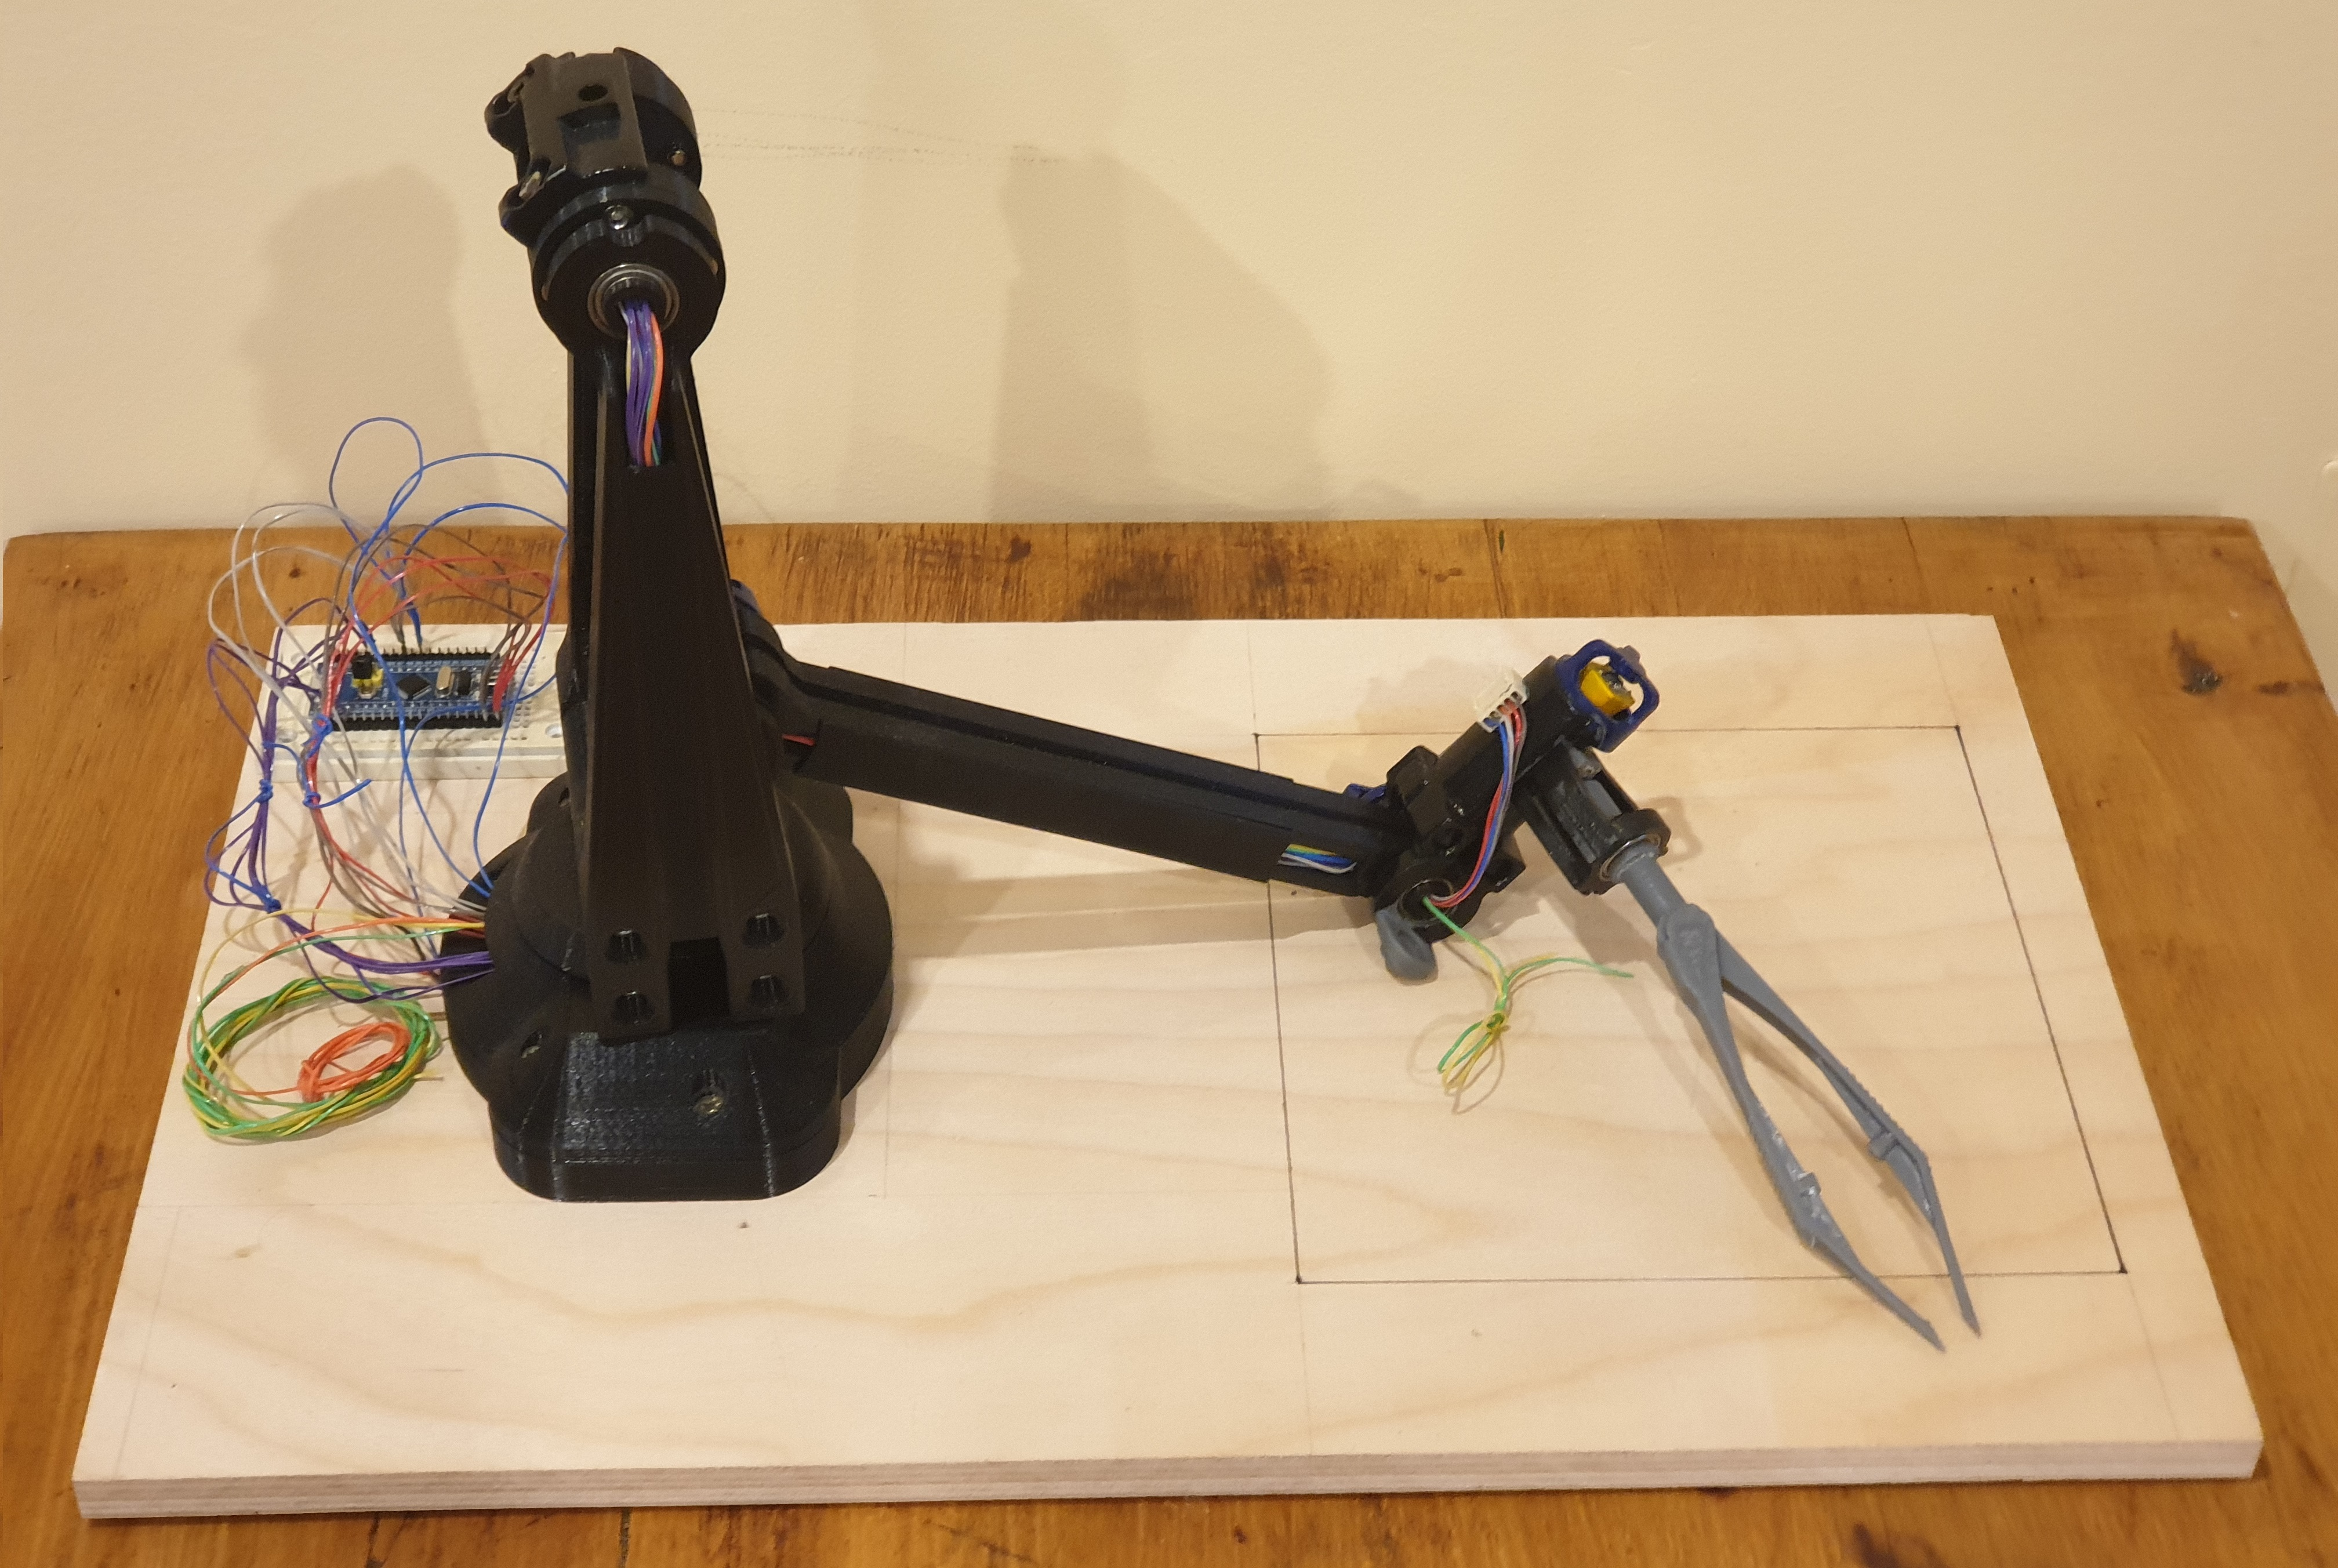
\includegraphics[width=150mm, keepaspectratio]{figures/Szakdoga/0_v_4_csipeszes}
\caption{Szakdolgozatomban elkészített telemanipuláto}
\label{fig:Szakdoga_csipeszes}
\end{figure}

Nagyon fontosnak tartottam, hogy a megtervezett eszközt el is készítsem valamilyen formában, mivel így sokkal alaposabban megtudtam vizsgálni az eszközt. A telemanipulátor 3D nyomtatással lett elkészítve. A FDM\footnote{Fused Deposition Modeling - A nyomtatási technológia a hőre lágyuló polimerekkel képes 3D-s objektumokat nyomtatni. Az FDM nyomtatók azzal az alapelvvel működnek, hogy szobahőmérsékleten szilárd hőre lágyuló polimert 180$^{\circ}$- 300$^{\circ}$C-ra melegítve ömledéket állapotba kerülnek és a kívánt helyre lehet juttatni lineáris vezetékrendszer segítségével.} technológiával készült, viszont néhány alkatrész, mint például a szenzortartó elkészítéséhez SLA\footnote{StereoLithography Apparatus - modellteret UV aktív gyantával tölti fel. A nyomtatási térben egy síklapra építi fel a tárgyat úgyhogy, az belemerül egy gyantával teli kádba, ahol a megfelelő rétegvastagságú folyékony gyanta réteget UV lézerrel térhálósítja és köti adhézióval az előző réteghez} módon működő nyomtatót használtam. 

